\documentclass[./main.tex]{subfiles}
%\externaldocument{/chapter1}
\begin{document}


Retomando las ideas del capítulo \ref{ch1}, las células madre embrionarias reciben estímulos de diferenciación principalmente a través del ligando FGF4, y procesan la información recibida a través de la activación de ERK. En el capítulo \ref{ch2} nos preguntamos cómo es la dinámica de activación de ERK en mESCs en condiciones de cultivo que mantienen la pluripotencia. Encontramos que la actividad de ERK tiene forma de oscilaciones intermitentes, es decir, intervalos de oscilaciones alternados con intervalos de silencio y pulsos aislados. Pero, ¿cómo cambian las principales propiedades dinámicas de las oscilaciones intermitentes de actividad de ERK ante perturbaciones experimentales?

Para responder a este interrogante, en la primera parte de este capítulo nos enfocamos en entender cómo se modifica la dinámica de activación de ERK en ESCs al exponer a la célula a distintas concentraciones controladas de FGF4. Primero presentamos un nuevo protocolo experimental para obtener series temporales de la dinámica de actividad de ERK para células estimuladas con distintas concentraciones definidas de ligando. Luego, aplicamos las herramientas de análisis desarrolladas en el capítulo anterior para analizar de manera cuantitativa qué características de la dinámica de activación de ERK cambian y cuáles se conservan ante distintas dosis de ligando. En la segunda parte de este capítulo estudiamos qué aspectos de la dinámica de ERK son propios de este estadío de diferenciación. Primero presentamos un protocolo experimental distinto para adquirir series temporales que nos permiten comparar la dinámica de activación de ERK en ESCs y en células madre epiblasto, y luego aplicamos las herramientas de análisis desarrolladas en el capítulo anterior para llevar a cabo esta comparación. 


\section{El estímulo extracelular controla la duración de los intervalos oscilatorios}
\sectionmark{FGF4 controla la duración de los intervalos oscilatorios}

Esta sección tiene como propósito entender cómo cambia la dinámica de activación de ERK en ESCs ante exponer células a distintas concentraciones controladas de FGF4. Para esto, es necesario desarrollar un protocolo experimental nuevo que nos permita controlar la dosis de ligando con el que se estimula a las células a partir de las que adquiriremos nuevas mediciones de la dinámica de activación de ERK. En este marco, nuestro sistema biológico de estudio serán las células madre embrionarias de ratón mutantes que no pueden producir su propio FGF4, que estimularemos con distintas concentraciones controladas de ligando que son relevantes a nivel biológico. Luego, implementaremos el protocolo de análisis de datos descripto en el capítulo anterior buscando entender cómo es el comportamiento de los observables que definimos previamente cuando estimulamos a las células con distintas dosis de FGF4, y qué propiedades dinámicas de las oscilaciones intermitentes de actividad de ERK cambian o se conservan en cada caso. 


\subsection{Células madre embrionarias mutantes en \textit{Fgf4}}
\label{sec:c2_KO}

%Buscábamos diseñar un protocolo experimental que nos permita adquirir series temporales de la dinámica de actividad de ERK en células estimuladas con distintas dosis controladas de FGF4. Con esta idea, primero introdujimos mESCs mutantes en \textit{Fgf4}, luego determinamos el rango de concentraciones a las que íbamos a estimular a las células mutantes, y finalmente estudiamos si la variabilidad de la activación de ERK que observamos en las células \textit{wild type} se conservaba en este nuevo sistema experimental. 

La señalización de FGF4 producido por las mismas células es el principal estímulo endógeno de la red de señalización FGF/ERK en ESCs. Entonces, para poder controlar la dosis de ligando con el que las células madre embrionarias eran estimuladas, era necesario anular la capacidad de las células de producir su propio FGF4. Para esto, introdujimos una mutación de pérdida de función del gen \textit{Fgf4} en la línea celular que tenía integrado el sensor de traslocación KTR (sección \ref{C2_ssec:sensor}). 


Observamos en filmaciones que células mutantes en \textit{Fgf4} fueron viables y continuaron dividiéndose en el medio N2B27, que es un medio químicamente definido que no contiene factores que estimulen la red de señalización FGF/ERK (\href{http://movie.biologists.com/video/10.1242/dev.199710/video-2}{película FGF}, sección \ref{C1_sec:ESC}). Este resultado es coherente con trabajos anteriores \cite{Kunath2007}, y demuestra que la señalización de FGF4 es prescindible para la progresión del ciclo celular en las ESCs. 


Para medir los niveles de activación de ERK en las células mutantes, utilizamos la técnica de \textit{\textit{Western blot}}.
\marginpar{\textit{Western Blot}} Esta técnica permite detectar una proteína dentro de una muestra biológica, y posibilita realizar comparaciones cuantitativas de los niveles de proteína entre diferentes muestras. En general, la proteína de interés es detectada mediante el uso de un anticuerpo que reconoce y se une a un epítopo propio de la misma. Luego, si esta proteína está presente en la muestra analizada, aparecerá una banda asociada en el revelado del experimento. Cuanto más intensa la banda, más proteína detectada.  


En este caso, el experimento fue diseñado para detectar ambas informas de ERK, ERK1 y ERK2, en sus versiones fosforiladas (es decir, activas) y totales (es decir, activas e inactivas) (figura \ref{C3_fig:FGF_mutante}A). Realizamos las mediciones en las células mutantes en varias condiciones experimentales, y como control utilizamos células \textit{wild type}. En el caso de las células cultivadas en s+L, observamos altos niveles de pERK en ambas poblaciones celulares. Este resultado era esperable, pues factores presentes en el medio de cultivo activan ERK (sección \ref{C1_sec:ESC}). En el caso de células cultivadas en N2B27 + Chiron, observamos que los niveles de pERK se redujeron fuertemente en la línea celular mutante. En esta condición no había factores en el medio de cultivo capaces de activar ERK, lo que verifica que el mutante no puede producir su propio FGF4 y, de esta manera, promover la activación de ERK. Por último, los niveles de pERK en mutantes en esta condición experimental eran similares a los de las células tratadas en el mismo medio de cultivo, pero con el inhibidor MEKi, insinuando que la mutación de pérdida que implementamos e inhibir químicamente proteína que activa a ERK en la red de señalización FGF/ERK tiene un impacto similar. 


En el capítulo anterior observamos que en las células \textit{wild type} tratadas con MEKi, el sensor KTR de traslocación se distribuía uniformemente (figura \ref{C2_fig:KTR}). En cambio, en el caso de las células mutantes, notamos que se localizaba preferentemente en el citoplasma (figura \ref{C3_fig:FGF_mutante}B). Atribuimos esta diferencia a que la privación crónica de FGF4 en la línea celular mutante conduce a un desplazamiento en la relación citoplasmática-nuclear del sensor, desplazamiento que es independiente de pERK. 



\begin{figure}
    \centering
    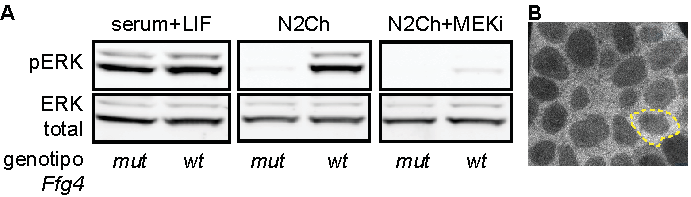
\includegraphics[width=1\columnwidth]{figures/chapter3/C3_FGF_mutant.pdf} 
    \caption{\textbf{Los niveles de pERK se redujeron fuertemente en células madre embrionarias mutantes.} (A) \textit{Western blot} para pERK y ERK total en células \textit{wild type} y mutantes de \textit{Fgf4} que crecen en las condiciones de medios indicadas, donde N2 es abreviatura de N2B27 y Ch de chiron. La banda superior corresponde a la isoforma ERK1, y la inferior a la isoforma ERK2 en cada caso. (B) Un cuadro de la película que expresa el sensor KTR de traslocación de pERK, integrado en células mutantes en \textit{Fgf4} y crecidas en N2B27. La línea amarilla discontinua indica el contorno de una célula.Los detalles del experimento se encuentran en \cite{Fabris2022}.}
    \label{C3_fig:FGF_mutante}
\end{figure}


Una vez establecidas las células madre embrionarias de ratón mutantes, planeamos estimularlas con distintas concentraciones controladas de ligando. En este marco, era necesario determinar qué concentraciones de FGF4 extracelular eran relevantes biológicamente. En otras palabras, era importante cubrir el rango dinámico (i) de la fosforilación de ERK a la respuesta de FGF4, y (ii) de la transcripción de un gen reportero que dependa de la red FGF/ERK. 


Para conocer el rango dinámico de la fosforilación de ERK en respuesta de FGF4, primero estudiamos el comportamiento de pERK en células mutantes con el sensor integrado bajo el estímulo de distintas concentraciones de FGF4. En la figura \ref{C3_fig:FGF}A presentamos los \textit{Western Blots} para pERK y ERK total para células mutantes estimuladas con distintas concentraciones de FGF4 extracelular. Podemos observar que la concentración de pERK aumenta conforme a la dosis de FGF4 extracelular, mientras que la concentración de ERK total se mantiene constante. En la figura \ref{C3_fig:FGF}B se encuentra cuantificada la figura \ref{C3_fig:FGF}A. Esta cuantificación se realizó utilizando el software FIJI/ImageJ, y para producirla se integraron las intensidades de las bandas de las isoformas ERK1 y ERK2 \cite{Rueden2017}. Podemos observar que pERK crece para concentraciones bajas de FGF4, y este crecimiento se aplana levemente luego de los $20$ ng/ml de estímulo extracelular. Este aplanamiento nos indica el rango dinámico de la fosforilación de ERK a la respuesta de FGF4.


Para conocer el rango dinámico de la transcripción de un gen reportero que dependa de la red FGF/ERK, medimos la transcripción de \textit{Sprouty4} (\textit{Spry4}) -un gen reportero que depende de pERK- ante el estímulo de distintas concentraciones de FGF4.\marginpar{citometría de\\flujo} Para esto, empleamos la técnica de citometría de flujo. Esta técnica permite contar la presencia de biomarcadores en un cultivo celular. En este caso, utilizamos una línea de mESCs con un reportero fluorescente insertado en el locus de \textit{Spry4} \cite{Morgani2018}. Con este diseño experimental, cuanto más fluorescencia observábamos, más actividad transcripcional de ERK hay. En la figura \ref{C3_fig:FGF}C notamos que la intensidad media de fluorescencia aumentaba conforme al estímulo extracelular, y siempre era mayor a los niveles adquiridos para el caso sin estímulo. En la figura \ref{C3_fig:FGF}D podemos ver la cuantificación de estas mediciones, que realizamos en FlowJo (BD Biosciences). En esta cuantificación, la actividad transcripcional de pERK crece de manera mucho más abrupta que la forma en la que crece la concentración de pERK ante distintas dosis de FGF4 extracelular (comparar paneles \ref{C3_fig:FGF}B y D). Sin embargo, el crecimiento de la actividad transcripcional se aplana luego de los $20$ ng/ml de estímulo extracelular, al igual que la fosforilación de ERK a la respuesta de FGF4. Este aplanamiento nos indica el rango dinámico del gen reportero \textit{Spry4}.

A partir de estos resultados, elegimos estimular la actividad de ERK en el rango de concentraciones de $2.5$ a $20$ ng/ml, intervalo que consideramos biológicamente relevante dado que abarca el rango dinámico de respuesta de FGF4 al nivel de pERK y de la transcripción de un gen reportero que depende de FGF/ERK. Además, en este intervalo de concentraciones elegidas también se aseguraba la diferenciación de las mESCs hacia el endodermo primitivo \cite{Raina2021}. Realizamos una inmunomarcación para distintas concentraciones de FGF4 en el rango que elegimos para estimular las células, donde observamos que la variabilidad que observamos en el capítulo anterior en las células \textit{wild type} en s+L se conservaba, lo que sugiere que la variabilidad de la activación de ERK en ESCs individuales no es producto de mantener a las células en condiciones de cultivo químicamente indefinidas, sino que probablemente sea producto de mecanismos intracelulares (ver apéndice \ref{C3_ap:inmuno}).


\begin{figure}
    \centering
    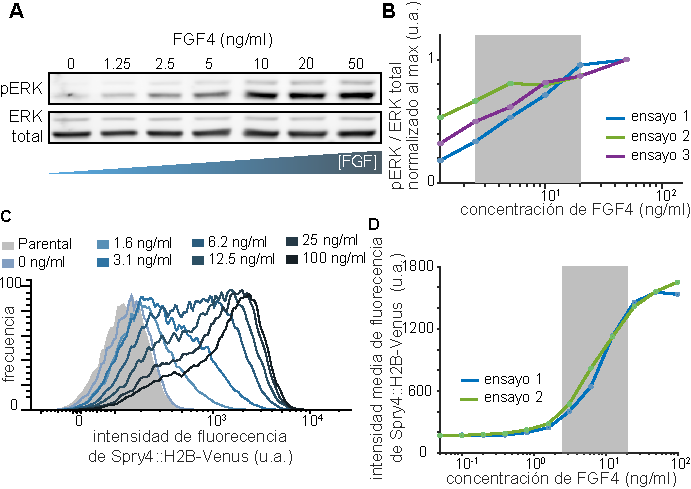
\includegraphics[width=1\columnwidth]{figures/chapter3/C3_FGF_conc.pdf} 
    \caption{
\textbf{Rango dinámico de señalización y respuesta transcripcional a dosis controladas de FGF4 en ESCs.} (A) \textit{Western Blot} representativo para pERK y ERK total en células mutantes de \textit{Fgf4} tratadas con un rango de concentraciones de FGF4, con el mismo protocolo experimental que en la figura \ref{C3_fig:FGF_mutante}. La banda superior corresponde a la isoforma ERK1, y la inferior a la isoforma ERK2 en cada caso.(B) Cuantificación de los datos de \textit{Western Blot} del panel A para N = 3 experimentos independientes. (C) Citometría de flujo de células Fgf4\textsuperscript{mutante}, Spry4\textsuperscript{H2B-Venus/+} estimuladas con un rango de concentraciones de FGF4. Se utilizó una línea no reportera como control negativo (sombra gris). Las frecuencias se normalizaron a la moda. (D) Cuantificación de la intensidad de fluorescencia media de H2B-Venus de C. El recuadro gris en B y D indica el rango de concentraciones de FGF4 de $2.5$ a $20$ ng/ml que utilizamos en este trabajo para estimular a células mutantes. Los detalles del experimento se encuentran en \cite{Fabris2022}.}
    \label{C3_fig:FGF}
\end{figure}


\subsection{Mediciones de la dinámica de actividad de ERK para dosis controladas de FGF4}


Una vez establecidas las condiciones experimentales, buscamos la manera de adquirir el estado estacionario de la actividad de ERK en células mutantes estimuladas con distintas concentraciones de FGF4, y que conserven la pluripotencia. Para que las células pudieran adaptarse a FGF4, primero pretratamos las células mutantes con el sensor de traslocación integrado con las correspondientes dosis de FGF4 en el medio N2B27 suplementado con chiron y LIF durante 24 horas, buscando mantener la pluripotencia. Como LIF puede activar ERK \cite{Ohtsuka2015}, 4 horas antes de comenzar las mediciones repusimos el medio N2B27 con chiron y FGF4 pero sin LIF (figura \ref{C3_fig:FGF_traces}A). Para registrar la localización del sensor en función del tiempo, filmamos a células con el sensor integrado con una resolución de $20$ segundos por cuadro y durante un máximo de $2$ horas (\href{http://movie.biologists.com/video/10.1242/dev.199710/video-2}{película FGF}). Si bien FGF4 promueve la diferenciación de ESCs hacia linajes embrionarios en condiciones de cultivo donde sólo hay uno de los tres factores del medio 2i+LIF, lo hace en $1$ ó $2$ días, una escala de tiempo mucho más lenta que las mediciones de aproximadamente dos horas que realizamos. Por este motivo consideramos que las células siguen siendo pluripotentes durante la medición \cite{Kalkan2017}. 


\begin{figure}
    \centering
    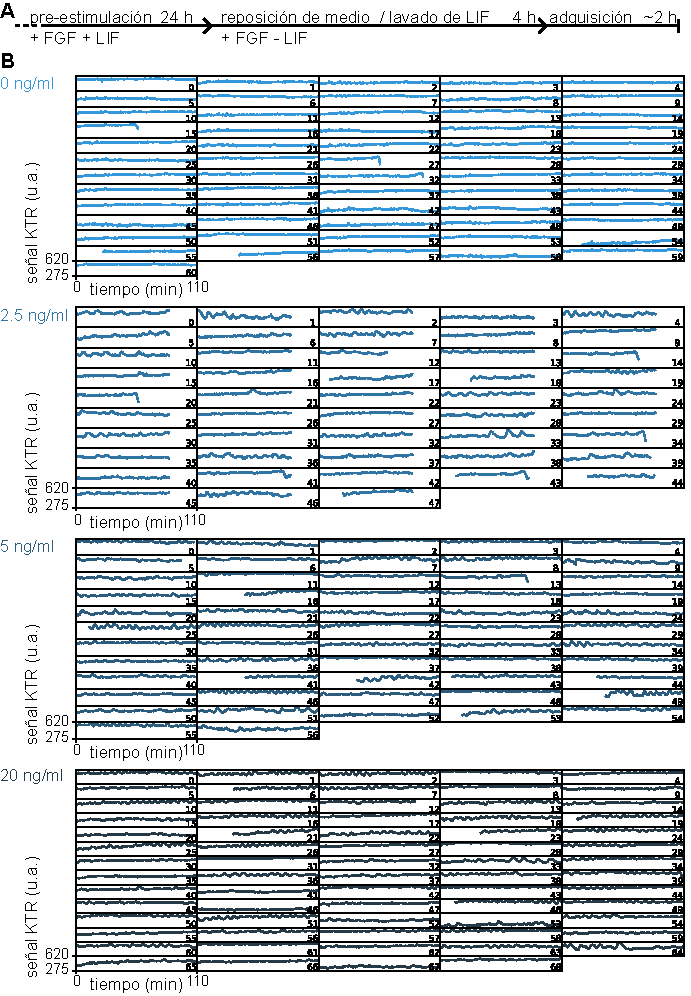
\includegraphics[width=1\columnwidth]{figures/chapter3/C3_FGF_traces.pdf} 
    \caption{ \textbf{Dinámica de la señal KTR adquirida para distintas dosis de FGF4.} (A) Esquema del protocolo experimental para medir la actividad dinámica de ERK en estado estacionario ante estimular mESCs pluripotentes mutantes en el gen \textit{Fgf4} con dosis definidas de FGF4. (B) Series temporales de la señal KTR obtenidas como la intensidad media de un ROI nuclear en la imagen invertida. La adquisición se realizó siguiendo el protocolo experimental representado en A., estimulando con distintas dosis de FGF4 indicadas arriba a la izquierda en cada caso. La disminución de la señal KTR al final de las trazas en las células 15, 27 y 32 (0 ng/ml), las células 14, 20, 34, 38, 41, 43 y 44 (2,5 ng/ml), la célula 13 (5 ng/ml) y las células 8 y 39 (20 ng/ml) se debe a la ruptura de la envoltura nuclear que sucede cuando las células entran en mitosis. Esta parte de las series temporales, junto con el pico inmediatamente anterior, se recortó para el análisis posterior. La tasa de adquisición fue de 20 s/cuadro. Los detalles del experimento se encuentran en \cite{Fabris2022}.}
    \label{C3_fig:FGF_traces}
\end{figure}

En ausencia de estímulo, en las filmaciones casi no observamos actividad pulsátil. En cambio, sí observamos una actividad pulsátil generalizada en todos los casos en donde estimulábamos a las células con FGF4, lo que sugiere que el FGF4 desencadena la actividad pulsátil de ERK (\href{http://movie.biologists.com/video/10.1242/dev.199710/video-2}{película FGF}). 

Para profundizar esta observación, obtuvimos series temporales que representen la dinámica de activación de ERK en cada condición a partir de realizar un \textit{tracking} de células individuales en las películas, realizando un procedimiento análogo al descripto en la sección \ref{C2_ssec:tracking}. En la figura \ref{C3_fig:FGF_traces}B presentamos los resultados de esta cuantificación. En las series temporales adquiridas a partir de medir células estimuladas con FGF4, observamos claramente actividad pulsátil, actividad que no observamos en las células sin estímulo de FGF4. Esta actividad pulsátil parecía tener un abanico de comportamientos dinámicos similar al que observamos en el capítulo \ref{ch2}. Además, parecía ser más activa conforme al aumento de FGF4 extracelular (comparar la condición $2.5$ con $20$ ng/ml). 


\subsection{Análisis cuantitativo de las series temporales}
\label{C3_ssec:analisis_cuantitativo}

Nuestra inspección visual nos sugería que la actividad pulsátil de actividad de ERK aumenta conforme aumenta el estímulo de FGF4, lo que nos motivó a preguntar qué rasgos dinámicos cambian y cuáles se conservan en las oscilaciones intermitentes de actividad dinámica de ERK al estimular a las células con distintas concentraciones de FGF4 extracelular. Para entender esto, realizamos un análisis cuantitativo de las series temporales de la figura \ref{C3_fig:FGF_traces}. Empleamos la estrategia de detección de pulsos descripta en la sección \ref{C2_sec:pulse_detection}, pero utilizando distintos parámetros de umbrales que elegimos para este nuevo conjunto de datos (ver cuadro \ref{C3_ap_tab:FGF_th}, apéndice \ref{C3_ap:FGF_pulse_detection}). Luego, implementamos un análisis similar al descripto en \ref{C2_sec:analisis}. 

Observamos que las distribuciones de amplitud de pulsos no eran significativamente diferentes entre las tres concentraciones estudiadas. Sin embargo, como la relación entre la amplitud de la señal adquirida del sensor de traslocación y la actividad dinámica de ERK es desconocida, por lo que no pudimos descartar tendencias en la amplitud de pulsos de actividad de ERK ante estimular a las células con  distintas dosis de ligando (apéndice \ref{ap_C3:amplitud}). 


En la figura \ref{C3_fig:FGF_actividad}A mostramos la fracción total de tiempo que las células individuales pulsaban. En todos los casos, observamos que la actividad pulsátil era heterogénea, resultado que iba en linea con el abanico de comportamientos dinámicos pulsátiles que observamos por inspección visual. Además, la fracción de tiempo promedio que las células pulsaban aumentaba con la concentración de FGF4 en el rango de 0 a 5 ng/ml, hasta niveles similares a los medidos en células \textit{wild type} en la condición con serum + LIF (figura \ref{C2_fig:actividad}). Este aumento en el promedio de la actividad pulsátil podría darse porque aumenta la cantidad de pulsos detectado en cada condición, o porque los pulsos tienen duraciones más largas. 


\begin{figure}
    \centering
    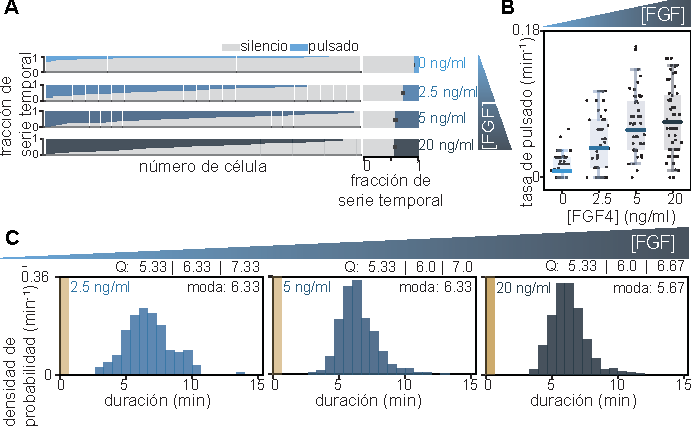
\includegraphics[width=1\columnwidth]{figures/chapter3/C3_FGF_activity.pdf} \caption{\textbf{La actividad pulsátil aumenta con FGF4 debido al aumento de la tasa de pulsado.} (A) Izquierda: fracción de tiempo que las células individuales estimuladas con diferentes concentraciones de FGF4 pasaron pulsando (azul), o sin pulsar (gris). Derecha: tiempo medio que las células de la población estuvieron pulsando (azul) o sin pulsar (gris). La barra de error indica SEM. (B) Tasa de pulsado para diferentes concentraciones de FGF4. Los puntos negros representan células individuales, las barras de color son la mediana, los límites de la caja son los percentiles 25 y 75 de las distribuciones, y los bigotes son los percentiles 5 y 95. (C) Distribuciones de la duración de pulsos para para cada condición experimental, donde células mutantes de \textit{Fgf4} fueron estimuladas con diferentes dosis de FGF4, indicadas arriba. El número de pulsos fue n = 164 (2,5 ng/ml), n = 426 (5 ng/ml) y n = 544 (20 ng/ml), y el número de células fue de N = 48 (2,5 ng/ml FGF4), N = 57 (5 ng/ml FGF4) y N = 69 (20 ng/ml FGF4). Se indican límite de resolución del reconocimiento de pulsos (barra amarilla) y los cuartiles (Q) 25, 50 y 75.}
    \label{C3_fig:FGF_actividad}
\end{figure}

Para estudiar cómo contribuía el número de pulsos a este aumento del tiempo de pulsado, definimos la \textbf{tasa de pulsado} de una célula como el número de pulsos dividido la duración de la serie temporal. En la figura \marginpar{tasa de pulsado} \ref{C3_fig:FGF_actividad}B mostramos la estadística de la tasa de pulsado en función de la concentración del estímulo, y encontramos que aumenta con la concentración de FGF4 en el mismo rango que la actividad. Este resultado podría explicar la observación de que el tiempo promedio en que las células pulsaban aumentaba con la dosis de FGF4. Sin embargo, la duración de los pulsos también podría influir en esta medida. 


Estudiamos cómo contribuía la duración de los pulsos al aumento de tiempo de pulsado. En el caso donde las células mutantes no fueron estimuladas con FGF4 no había suficiente estadística y decidimos no incluirla en el análisis. Sorprendentemente, las distribuciones de las duraciones de pulsos se solapaban entre las tres concentraciones de FGF4, y sus valores modales se conservaban (figura \ref{C3_fig:FGF_actividad}C). Para formalizar esta observación, implementamos el test de Kolmogorov-Smirnov para dos muestras para comparar las distribuciones entre sí \cite{Frodesen1979} (apéndice \ref{C3_ap:FGF_KS_test}).\marginpar{Test de Kolmogorov-Smirnov} El coeficiente $p$ que calcula este test es una medida de indistiguibilidad entre dos distribuciones: cuanto más indistinguibles son las dos distribuciones que se comparan, el valor de $p$ se acerca más a cero. Por el contrario, cuanto más distinguibles son, $p$  es más cercano a $1$. Observamos una tendencia sutil hacia distribuciones más estrechas con concentraciones más altas de FGF4, aunque el test de Kolmogorov indicaba que éstas eran significativamente diferentes sólo entre las condiciones de $2.5$ ng/ml y 20 ng/ml (cuadro \ref{C3_ap_tab:KS}). En definitiva, el aumento del tiempo de pulsado se debe mayoritariamente a un aumento en la tasa de pulsado y no a un aumento en la duración de pulsos. 


Luego nos preguntamos cómo se organizaban los pulsos en las series temporales en cada condición experimental. En la figura \ref{C3_fig:FGF_consecutive}A mostramos las distribuciones de intervalo de interpulsado. En consonancia con la conservación de la duración de pulso a lo largo de las concentraciones estudiadas, las distribuciones de IPI tenían un valor modal similar de unos 7 min. en todas las condiciones. Sin embargo, las distribuciones eran más estrechas a medida que aumentaba la concentración de FGF4, con una clara diferencia significativa entre $2.5$ y 20 ng/ml de FGF4 (figura \ref{C3_fig:FGF_consecutive}A, cuadro \ref{C3_ap_tab:KS}). Que las distribuciones de tiempo de interpulsado sean más estrechas indican mayor frecuencia de IPIs pequeños y menor frecuencia de IPIs más largos. Que los intervalos de interpulsado sean cada vez más pequeños, y del orden de la duración de los pulsos, sugiere una dinámica pulsátil cada vez más regular.  


\begin{figure}
    \centering
    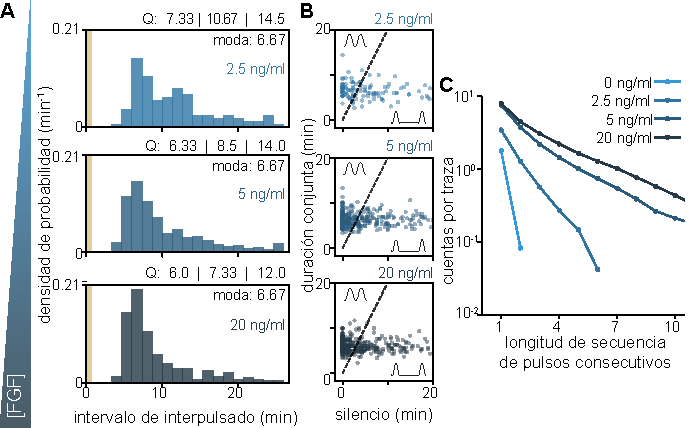
\includegraphics[width=1\columnwidth]{figures/chapter3/C3_FGF_consecutive.pdf} \caption{\textbf{La regularidad de la actividad pulsátil aumenta con las concentración de FGF4.} (A) Distribuciones de los intervalos de interpulsado entre pares de pulsos sucesivos para para cada condición experimental, donde células mutantes de \textit{Fgf4} fueron estimuladas con diferentes dosis de FGF4, indicadas a la derecha. El número de pulsos detectados fue de n = 124 (2,5 ng/ml), n = 370 (5 ng/ml) y n = 479 (20 ng/ml). El límite de resolución del reconocimiento de pulsos (barra amarilla) y los cuartiles (Q) 25, 50 y 75 se indican en B. (B) Duración conjunta de los pulsos en función de a los intervalos de silencio para pares de pulsos sucesivos para para cada condición experimental, donde células mutantes de \textit{Fgf4} fueron estimuladas con diferentes dosis de FGF4, indicadas arriba. La línea discontinua de pendiente 2 clasifica los pares de pulsos en consecutivos (arriba) y no consecutivos (abajo). El rango de los ejes se ajustó para resolver mejor los puntos de datos individuales, dejando fuera de la escala 6 de 124 (2,5 ng/ml FGF4), 26 de 370 (5 ng/ml FGF4) y 33 de 479 (20 ng/ml FGF4) puntos de datos. (D) Frecuencia de trenes de pulsos consecutivos en función de la cantidad de pulsos que componen el tren para diferentes dosis de FGF4, determinado como en la figura \ref{C2_fig:seq_pulsos_consecutivos}B. Número de células en A-D es N = 61 (0 ng/ml FGF4), N = 48 (2,5 ng/ml FGF4), N = 57 (5 ng/ml FGF4) y N = 69 (20 ng/ml FGF4).}
    \label{C3_fig:FGF_consecutive}
\end{figure}
 

Para evaluar el aumento de la regularidad de la actividad pulsátil, graficamos la duración conjunta de pulsos sucesivos en función de la duración del intervalo de silencio entre ellos para calcular la proporción de pares de pulsos consecutivos en cada concentración de FGF4 extracelular (figura \ref{C3_fig:FGF_consecutive}B). La proporción de pares de pulsos consecutivos aumentó de forma constante en todo el rango de concentración de FGF, siendo $49,2 \% $ para $2.5$ ng/ml, luego $57.6\%$ para 5 ng/ml, y finalmente $63.9\%$ para 20 ng/ml de FGF4. En linea con esta observación, en la figura \ref{C3_fig:FGF_consecutive}C observamos que las secuencias más largas de pulsos consecutivos también eran más prevalentes a dosis más altas de FGF4.


En resumen, encontramos que FGF4 desencadena la actividad pulsátil de ERK. Esta actividad es heterogénea, independientemente de la dosis de ligando, pero en promedio aumenta conforme a la dosis de FGF4. La duración de los pulsos parece no tener una fuerte dependencia del estímulo celular, y el aumento en la actividad parece tener origen en que la tasa de pulsado aumenta conforme al estímulo de FGF4. A medida que aumenta la concentración de FGF4, encontramos que la actividad pulsátil aumenta su regularidad, dando lugar a secuencias de pulsos consecutivos más largas. Concluyendo, estos resultados nos sugieren que FGF4 controla la duración de los intervalos oscilatorios de las oscilaciones intermitentes de ERK en ESCs pluripotentes.


\section{Las oscilaciones intermitentes son menos prevalentes en células más diferenciadas}
\sectionmark{Las oscilaciones intermitentes son menos prevalentes en EpiSCs}

Esta sección tiene como propósito evaluar qué aspectos dinámicos de las oscilaciones intermitentes de actividad de ERK son propios del estadío de diferenciación de las células madre embrionarias. Abordamos esta pregunta comparando la dinámica de activación de ERK en células madre embrionarias con células madre epiblasto, un tipo celular levemente más diferenciado (sección \ref{C1_sec:EpiSCs}). Para realizar esta comparación, primero discutimos un protocolo experimental que nos permita realizar mediciones de la dinámica de actividad de ERK en ambos tipos celulares simultáneamente y en las mismas condiciones experimentales. Luego, implementamos el protocolo de análisis de datos descripto en el capítulo anterior para entender cómo se comportan los observables que caracterizan las oscilaciones intermitentes de actividad de ERK en cada caso. 


\subsection{Adquisición de series temporales de la dinámica de ERK en células madre epiblasto}

Para obtener un tipo celular más diferenciado, transicionamos las ESCs \textit{wild type} de ratón con el sensor KTR integrado hacia un estado de células madre epiblasto cultivándolas durante al menos 9 pasajes en N2B27 suplementado con FGF2 y Activina (sección \ref{C1_sec:ESC}) \cite{Guo2009}. Para obtener cultivos más homogéneos, añadimos el inhibidor de Wnt XAV939, clave para mantener los cultivos indiferenciados (medio FAX).


A continuación, queríamos comparar la dinámica de activación de ERK en ambos tipos celulares: EpiScs y ESCs. Normalmente, a estos dos tipos celulares se los mantiene en cultivo en medios diferentes, elegidos para conservar las células indiferenciadas (sección \ref{C1_sec:ESC}). Esto presenta una limitación experimental importante puesto que al comparar la dinámica de activación de ERK en EpiSCs crecidas en FAX con la de ESCs crecidas en serum + LIF, cualquier cambio que observáramos podría deberse a una diferencia entre los tipos celulares, o ser una consecuencia de alguna diferencia entre los medios de cultivo. Para distinguir entre estas dos posibilidades, decidimos comparar la dinámica de ERK en las EpiSCs con la de las ESCs transferidas a medio FAX poco antes del inicio de la medición.


Para registrar la localización del sensor en función del tiempo, filmamos a ambos tipos celulares con el sensor integrado con una resolución de $20$ segundos por cuadro y durante un máximo de casi $4$ horas. Las condiciones experimentales que consideramos fueron EpiSCs que crecían en FAX con o sin MEKi, y ESCs en FAX también con o sin MEKi (\href{http://movie.biologists.com/video/10.1242/dev.199710/video-3}{película EpiSCs}, figura \ref{C3_fig:EPI_traces}A). En ambos tipos celulares observamos actividad pulsátil de ERK cuando las células crecían en FAX, actividad que no observamos en las condiciones con MEKi (\href{http://movie.biologists.com/video/10.1242/dev.199710/video-3}{película EpiSCs}).


Profundizando, obtuvimos series temporales que representen la dinámica de activación de ERK en cada condición a partir de realizar un \textit{tracking} de células individuales en las películas, realizando un procedimiento análogo al descripto en la sección \ref{C2_ssec:tracking}. En la figura \ref{C3_fig:EPI_traces}B mostramos el resultado de estos seguimientos, que confirman la existencia de actividad pulsátil para ambos tipos celulares crecidos en FAX, actividad que desaparece ante la presencia del inhibidor MEKi. 


\begin{figure}
    \centering
    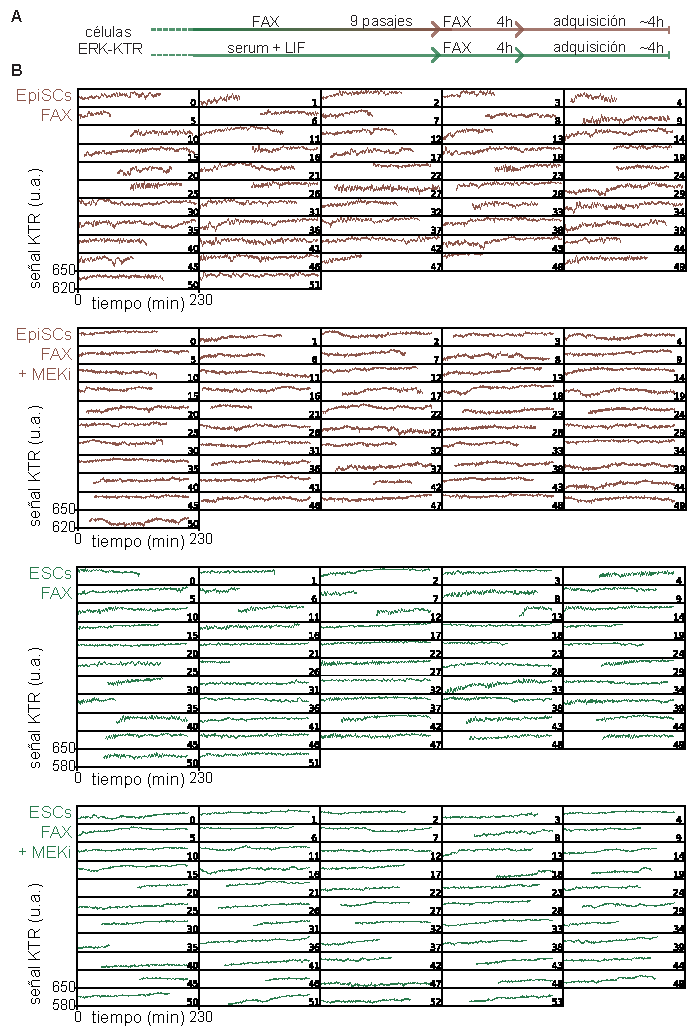
\includegraphics[width=1\columnwidth]{figures/chapter3/C3_EpiSC_traces.pdf} \caption{\textbf{Dinámica de la señal KTR en EpiSCs y ESCs creciendo en FAX.} (A) Esquema del protocolo experimental diseñado para comparar las características dinámicas de la actividad de ERK en ESCs y EpiSCs creciendo en el mismo medio. (B) Series temporales de la señal KTR obtenidas como la intensidad media de una ROI nuclear en la imagen invertida en EpiSCs o ESCs individuales, creciendo en FAX con o sin MEKi según se indica arriba a la izquierda en cada caso. La disminución de la señal KTR al final de las trazas de EpiSC 27 y de la ESC 1 de ESC que crecían en FAX sin MEKi se debe a la ruptura de la envoltura nuclear cuando las células entran en mitosis. Esta parte de la serie temporal, junto con el pico inmediatamente anterior, se recortó para el análisis posterior. La tasa de adquisición fue de 20 s/cuadro.}
    \label{C3_fig:EPI_traces}
\end{figure}


\subsection{Análisis cuantitativo de las series temporales}

Para realizar una comparación cuantitativa de las series temporales de la figura \ref{C3_fig:EPI_traces}B, empleamos una estrategia de detección de pulsos descripta en la sección \ref{C2_sec:pulse_detection}. Para cada tipo celular, elegimos nuevos parámetros umbrales que se encuentran detallados en el cuadro \ref{C3_ap_tab:EPI_th} (apéndice \ref{C3_ap:EPI_pulse_detection}). A continuación, implementamos un análisis similar al descripto en \ref{C2_sec:analisis}. 


En la figura \ref{C3_fig:EPI_activity}A encontramos que las dinámicas pulsátiles eran heterogéneas en ambas condiciones, pero la fracción de tiempo en que las células estaban pulsando era menor para las EpiSCs que para las ESCs. Además, la figura \ref{C3_fig:EPI_activity}B nos indicó que la duración media de pulsos era ligeramente mayor en las EpiSCs en comparación con las ESCs. En definitiva, para el caso de las EpiSCs la fracción de tiempo que las células pulsaban en promedio era menor y la duración de pulsos media era mayor que en el caso de las ESCs. Estas observaciones sugieren que los pulsos eran menos frecuentes en las EpiSCs que en las ESCs. 

\begin{figure}
    \centering
    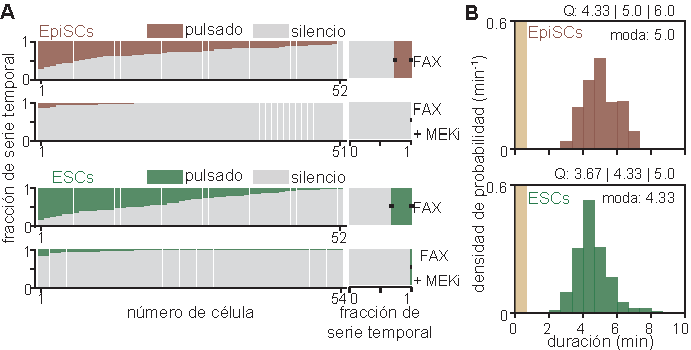
\includegraphics[width=1\columnwidth]{figures/chapter3/C3_EpiSC_activity.pdf} \caption{\textbf{Los pulsos son menos frecuentes en células madre epiblasto.} (A) Izquierda: fracción de tiempo que las células individuales pulsaban (marrón para EpiSCs, verde para ESCs) o sin pulsar (gris) en FAX solo (arriba) o al añadir MEKi (abajo). Derecha: tiempo medio que las células pulsaban (marrón para EpiSCs, verde para ESCs) o no pulsaban (gris) en la población celular. La barra de error indica la media estándar. (B) Distribución de la duración de pulsos para las EpiSCs (arriba, marrón, $n = 402$ pulsos) y las ESCs (abajo, verde, $n = 588$ pulsos). Se indica el límite de resolución del reconocimiento de pulsos (barra amarilla) y los cuartiles (Q) 25, 50 y 75.}
    \label{C3_fig:EPI_activity}
\end{figure}


Las distribuciones de intervalo de interpulsado revelaron aún mayores diferencias entre los dos tipos celulares considerados. Mientras que la moda de la distribución del IPI era de $5.33$ minutos en las EpiSCs, en la ESCs era de sólo $4$ minutos, indicando que la tasa de pulsado era más lenta en las EpiSCs que en las ESCs (figura \ref{C3_fig:EPI_consecutive}A). Además, al ser la duración de pulsos menor, los pulsos parecen estar sistemáticamente más separados en las EpiSCs que en las ESCs. Complementando esta observación, los IPIs estaban más estrechamente distribuidos en las ESCs en comparación con las EpiSCs, sugiriendo que la actividad pulsátil era menos regular en las células más diferenciadas. Esta diferencia en la regularidad de actividad pulsátil fue confirmada ante evaluar la proporción de pares de pulsos consecutivos en cada caso (figura \ref{C3_fig:EPI_consecutive}B). Nuestras mediciones nos informaron que el $65.6\%$ de todos los pares de pulsos eran consecutivos en las ESCs, en contraste con sólo el $45,9\%$ en las EpiSCs. Ahondando en esta propiedad, observamos que las secuencias más largas de pulsos consecutivos eran más frecuentes en las ESCs en comparación con las EpiSCs (figura \ref{C3_fig:EPI_consecutive}C, arriba). Tanto para las EpiSCs como para las ESCs, las secuencias más largas de pulsos consecutivos fueron también más abundantes en los datos en comparación con un modelo de pulsado estocástico heterogéneo, en el que los pulsos mezclados aleatoriamente en las series temporales individuales (figura \ref{C3_fig:EPI_consecutive}C). 


\begin{figure}
    \centering
    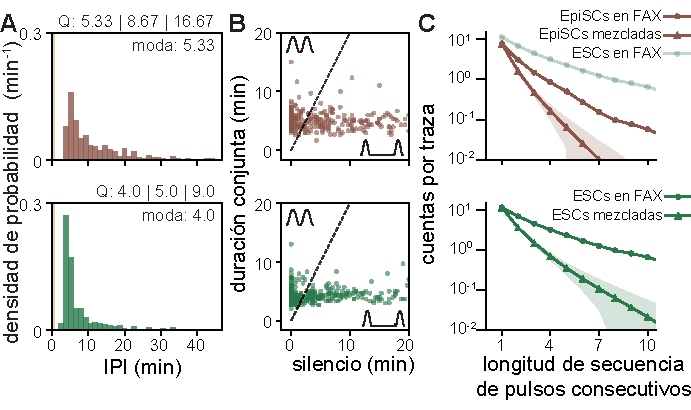
\includegraphics[width=1\columnwidth]{figures/chapter3/C3_EpiSC_consecutive.pdf} \caption{\textbf{Los intervalos oscilatorios de las oscilaciones intermitentes de ERK son menos frecuentes en células más diferenciadas.} (A) Distribución del intervalo de interpulsado para EpiSCs (arriba, marrón, n = 351 pares de pulsos) y ESCs (abajo, verde, n = 540 pares de pulsos). Se indican el límite de resolución del reconocimiento de pulsos (barra amarilla) y los cuartiles (Q) 25, 50 y 75. (B) Duración conjunta de los pulsos en función de los intervalos de silencio para pares de pulsos sucesivos en EpiSCs (arriba, marrón) y ESCs (abajo, verde). La línea discontinua con pendiente 2 clasifica los pares de pulsos en consecutivos (arriba) y no consecutivos (abajo). El rango de los ejes se ajustó para resolver mejor los puntos de datos individuales, dejando fuera de la escala 45 de 351 puntos de datos para EpiSCs, y 36 de 540 puntos de datos para ESCs. (C) Frecuencia de trenes de pulsos consecutivos en función del número de pulsos del tren. Arriba: Datos de EpiSCs (puntos marrones), datos de ESCs (puntos verdes) y modelo de población heterogénea para los datos de EpiSCs (triángulos marrones). Abajo: Datos de ESCs (puntos verdes, igual que arriba) y modelo de población heterogénea para los datos de ESCs (triángulos verdes). El área sombreada es la desviación estándar de 200 realizaciones independientes de los modelos estocásticos. Datos en A-C de N = 52 células en FAX para cada tipo celular.}
    \label{C3_fig:EPI_consecutive}
\end{figure}


En resumen, observamos actividad pulsátil de actividad de ERK en EpiSCs. Esta actividad era heterogénea, al igual que la detectada en las ESCs. Encontramos que la fracción de tiempo que las células pulsaban en promedio era menor en las EpiSCs que en las ESCs y la duración de pulsos era mayor, indicando que los pulsos son menos frecuentes en células levemente más diferenciadas que las ESCs. Además, comparando la distribución de IPIs y la proporción de pares de pulsos consecutivos, encontramos que la actividad pulsátil era menos regular en las EpiSCs. Esta observación se correspondía con que las secuencias más largas de pulsos consecutivos fueron menos frecuentes en las EpiSCs que en las ESCs. Sin embargo, éstas eran más abundantes en los datos experimentales que en datos obtenidos a partir de un modelo de pulsado estocástico heterogéneo simple. A pesar de las diferencias que encontramos en la dinámica de activación de ERK entre los distintos tipos celulares, nuestros resultados sugieren que la dinámica de activación de ERK en EpiSCs es compatible con oscilaciones intermitentes, como en el caso de las ESCs.


\section{Conclusiones y discusión}


En este capítulo estudiamos cómo cambian las principales propiedades de la dinámica de activación de ERK, las oscilaciones intermitentes, ante perturbaciones experimentales. Primero nos enfocamos en entender cómo se modifica la dinámica de activación de ERK en ESCs ante exponer a la célula a distintas concentraciones controladas de FGF4, y luego en qué aspectos de la dinámica de ERK son propios de este estadío de diferenciación.


Para entender cómo cambia la dinámica de activación de ERK en ESCs ante exponer células a distintas concentraciones controladas de FGF4, introdujimos mESCs mutantes en \textit{Fgf4}. Observamos que la mutación de pérdida que implementamos tenía un impacto similar sobre la activación de ERK que inhibir químicamente MEK, la proteína que activa a ERK en la red de señalización FGF/ERK (figura \ref{C3_fig:FGF_mutante}). Luego, estimulamos las células mutantes con distintas concentraciones controladas de ligando que cubrían el rango dinámico de la fosforilación de ERK a la respuesta de FGF4, y de la transcripción de \textit{Spr4}, un gen reportero que depende de la red FGF/ERK (figura \ref{C3_fig:FGF}). Finalmente, registramos la localización del sensor en función del tiempo que reportaba la dinámica de activación de ERK en su estado estacionario, y cuantificamos estas filmaciones para obtener series temporales de la dinámica de activación de ERK en células mutantes estimuladas con distintas dosis de FGF4 (figura \ref{C3_fig:FGF_traces}). Observamos actividad pulsátil de ERK en las células estimuladas con FGF4, actividad que no se percibía en ausencia de estímulo, lo que sugería que FGF4 desencadena la actividad pulsátil de ERK. 

%actividad
Aplicamos el algoritmo de detección de pulsos y la estrategia de análisis desarrollada en el capítulo anterior. Observamos que en promedio la fracción total de tiempo que las células individuales pulsaban aumentaba con la dosis de FGF4 (figura \ref{C3_fig:FGF_actividad}). Por otro lado, la duración de pulsos se mantenía para todas las condiciones, y este aumento en la actividad tenía origen en que aumentaba la tasa de pulsado. 


%regularidad
En otros tipos celulares que muestran que la dinámica de activación de ERK es en forma de pulsado estocástico, el aumento de los niveles de ligando conduce a intervalos más cortos entre los pulsos y, por lo tanto, a un aumento en la tasa de pulsado \cite{Albeck2013}. Esto se ha interpretado como una codificación de la concentración de ligando a través de la modulación de la frecuencia \cite{Li2019}. Nuestras observaciones en ESCs sugieren que es poco probable que se aplique el modelo de codificación modulada por frecuencia propuesto para otros tipos celulares en este caso. En este caso, observamos que distribución de intervalo de interpulsado conservaba su valor modal a medida que aumentaba el estímulo, pero era más estrecha, indicando una pulsación más regular. En la misma linea, nuestros resultados también mostraron que la proporción de pares de pulsos consecutivos aumentaba conforme a la dosis de FGF4 extracelular, así como la frecuencia de secuencias de pulsos consecutivos. Estas observaciones sugieren que FGF4 controla la duración de los intervalos oscilatorios de las oscilaciones intermitentes de ERK en ESCs. 


%%%%%%%%%%%%%%%%%%%%%%%%%%%%%%%%%%%%%%%%%%%%%%%%%%%%%%%%%%%%%%%%%%%
%%%%%%%%%%%%%%%%%%%%%%%%%%%%%%%%%%%%%%%%%%%%%%%%%%%%%%%%%%%%%%%%%%%
Para entender qué aspectos de la dinámica de ERK son propios de este estadío de diferenciación, comparamos la dinámica de activación de ERK en ESCs y EpiSCs, un tipo celular más diferenciado. Para realizarla, efectuamos filmaciones de la localización del sensor KTR en el tiempo para ambos tipos celulares, que luego cuantificamos (figura \ref{C3_fig:EPI_traces}). Utilizamos el mismo medio de cultivo en ambos casos para evitar posibles diferencias que provengan de utilizar distintos medios.

%menos pulsos
Aplicamos el algoritmo de detección de pulsos y la estrategia de análisis desarrollada en el capítulo anterior. A parir de este análisis, encontramos que las células más diferenciadas pulsaban, en promedio, durante un período de tiempo más corto (figura \ref{C3_fig:EPI_activity}). Además, las duraciones de pulso eran más largas comparadas con las ESCs. Estos resultados sugieren que los pulsos eran menos frecuentes en las EpiSCs que en las ESCs, lo que es consistente con los valores modales de IPI mayores en EpiSCs que en ESCs, como observamos. 

%menos regularidad
Además, observamos que los IPIs estaban más estrechamente distribuidos en las ESCs en comparación con las EpiSCs, sugiriendo que la actividad pulsátil era menos regular en las células más diferenciadas. Esta observación va en linea con que la menor proporción de pares de pulsos consecutivos y los trenes de pulsos de determinada duración menos frecuentes que observamos en EpiSCs en comparación con las ESCs (figura \ref{C3_fig:EPI_consecutive}). Con estos resultados, entendemos que las propiedades dinámicas de los pulsos de ERK dependen del estado de diferenciación. Por otra parte, nuestros resultados mostraron que la dinámica de ERK tanto en EpiSCs como en ESCs era inconsistente con escenarios de pulsado estocástico simples, lo que nos infiere que a señalización de ERK en ambos tipos celulares puede operar en un régimen dinámico similar. 

%las oscilaciones vienen de la red
Tanto la estimulación por parte del ligando que producen las mismas células como de FGF4 recombinante de las ESCs desencadenan actividad oscilatoria de ERK con escalas de tiempo similares en cuanto a la duración de los pulsos y su intervalo de interpulsado. Esto indica que las oscilaciones surgen en la red de transducción de señales intracelulares, de forma similar a la situación en otras líneas celulares \cite{Sparta2015}. Por otro lado, los pulsos de ERK eran más rápidos cuando las ESCs crecían en FAX en lugar de en serum+LIF (comparar la figura \ref{C3_fig:EPI_activity}B con \ref{C2_fig:amp_durac}C). Esto indica que los componentes del medio pueden afectar a las características dinámicas de la actividad de ERK. 

%heterogeneidad
La heterogeneidad en la fracción de tiempo que las células individuales pulsaban observada en ESCs crecidas en s+L (figura \ref{C2_fig:actividad}) también aparecía para dosis controladas de FGF4, e incluso en células más diferenciadas como las EpiSCs (figuras \ref{C3_fig:FGF_actividad}, \ref{C3_fig:EPI_activity}). Como insinuamos previamente, la heterogeneidad que observamos en la dinámica de activación de ERK en ESCs podría ser relevante para profundizar en la comprensión sobre decisiones del destino celular en las células pluripotentes. Esta observación podría resultar de diferencias estables en el comportamiento dinámico entre las células, o de que las células individuales tengan transiciones de estados oscilatorios activos e inactivos en escalas temporales largas en comparación con las mediciones. En el próximo capítulo exploramos estas posibilidades. 


\end{document}